\documentclass[dvipdfmx,uplatex]{jsarticle}

\usepackage[backend=biber,style=ieee]{biblatex}
\addbibresource{sample.bib} % bibファイル

\usepackage{inouelab} % 井上研製ライブラリ
\usepackage{titlesec} % 改ページ
\usepackage{amsmath,amssymb} % 数式
\usepackage{bm} % ベクトル
\usepackage{url} % リンク
\usepackage{here} % 図版配置用
\usepackage[dvipdfmx]{graphicx} % 図
\usepackage{tabularx} % 表
\usepackage{multirow} % 表
\usepackage{booktabs} % 表
\usepackage{pdfpages} % PDF

\def\refeq#1{(\ref{#1})} % 式参照用
\def\rm#1{\mathrm{#1}} % 立体
\allowdisplaybreaks % 式がページまたぐ用

\makeatletter
  % 章ごとに改ページさせる
  \newcommand{\sectionbreak}{\clearpage}

  % 番号をつけるルール変更
  \renewcommand{\theequation}{%
    \thesection.\arabic{equation}}
  \@addtoreset{equation}{section}
  \renewcommand{\thefigure}{%
    \thesection.\arabic{figure}}
  \@addtoreset{figure}{section}
  \renewcommand{\thetable}{%
    \thesection.\arabic{table}}
  \@addtoreset{table}{section}
\makeatother

\begin{document} % 本文開始

%% タイトルページ
\pagestyle{empty} % ページ番号を記述しない
\title{\vspace{20mm} \huge{タイトル}}
\author{\vspace*{1mm}\ \\早稲田大学先進理工学研究科 電気・情報生命工学科\\研究指導名:確率的情報処理\\指導教員名:井上真郷\\学籍番号:\\氏名:}
\date{\vspace*{1mm}\ \today}
\maketitle % タイトルを出力
\clearpage % 改ページ

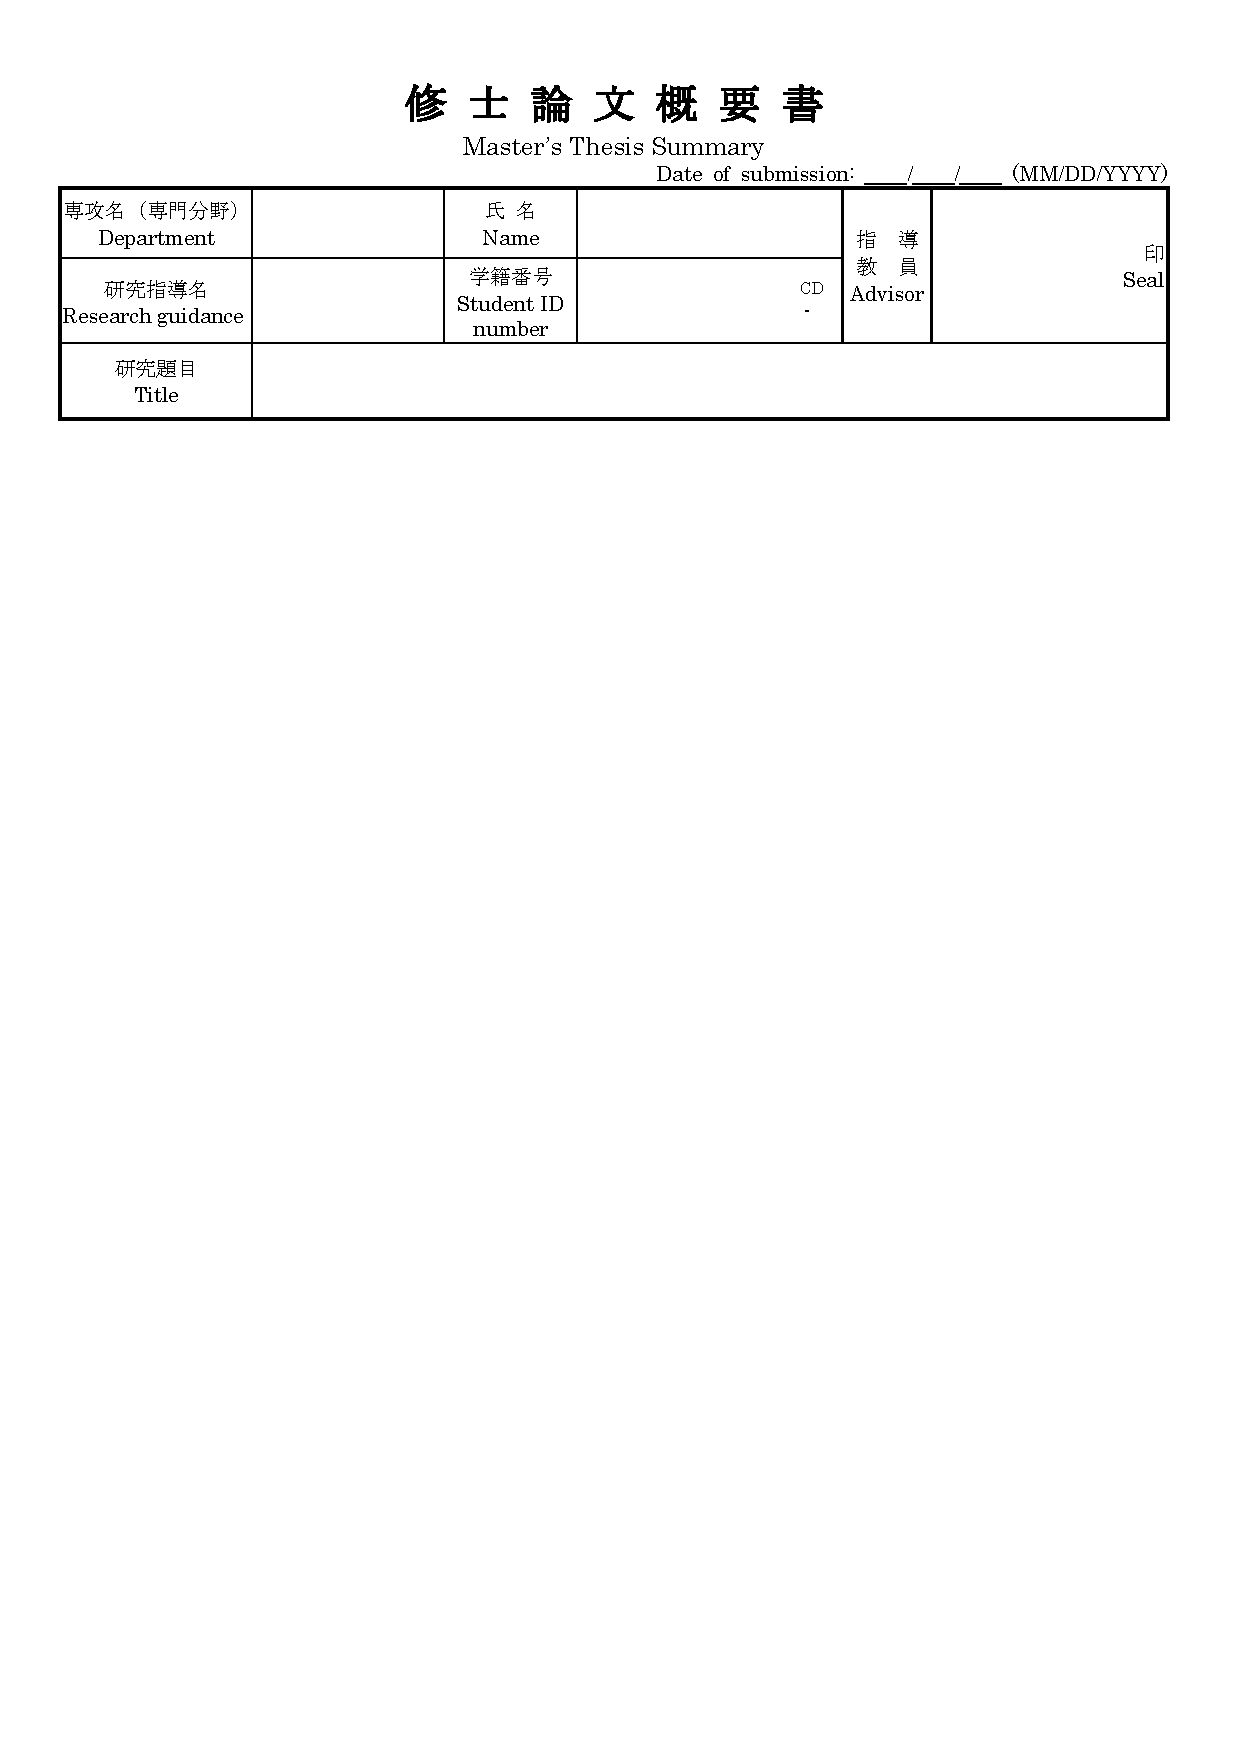
\includepdf[pages=-]{extra/gaiyou.pdf} % 誓約書を挿入

%% 目次
\setcounter{page}{1} % ここが1ページ目
\pagestyle{plain} % フッターにページ番号を出力する
\setcounter{tocdepth}{3}
\tableofcontents % 目次を出力
\clearpage % 改ページ

\section{サンプル}\label{sec:sample}

\ref{sec:sample} では

\subsection{画像}

図\ref{fig:logo}に示す

\begin{figure}[H] % 画像出力
  \begin{center}
    
\includegraphics[width=50mm]{fig/logo.png}
    \caption{井上 wiki のロゴ}
    \label{fig:logo}
  \end{center}
\end{figure}

\subsection{数式}

式\refeq{equ:alpha}に示す

\begin{equation} % 数式出力
  \alpha
  \label{equ:alpha}
\end{equation}

\subsection{文献}

Grad-Cam \cite{Selvaraju_2019} は〜.

\section*{謝辞} % *で章/節番号を振らない

\clearpage

\printbibliography[title=参考文献] % 参考文献を表示

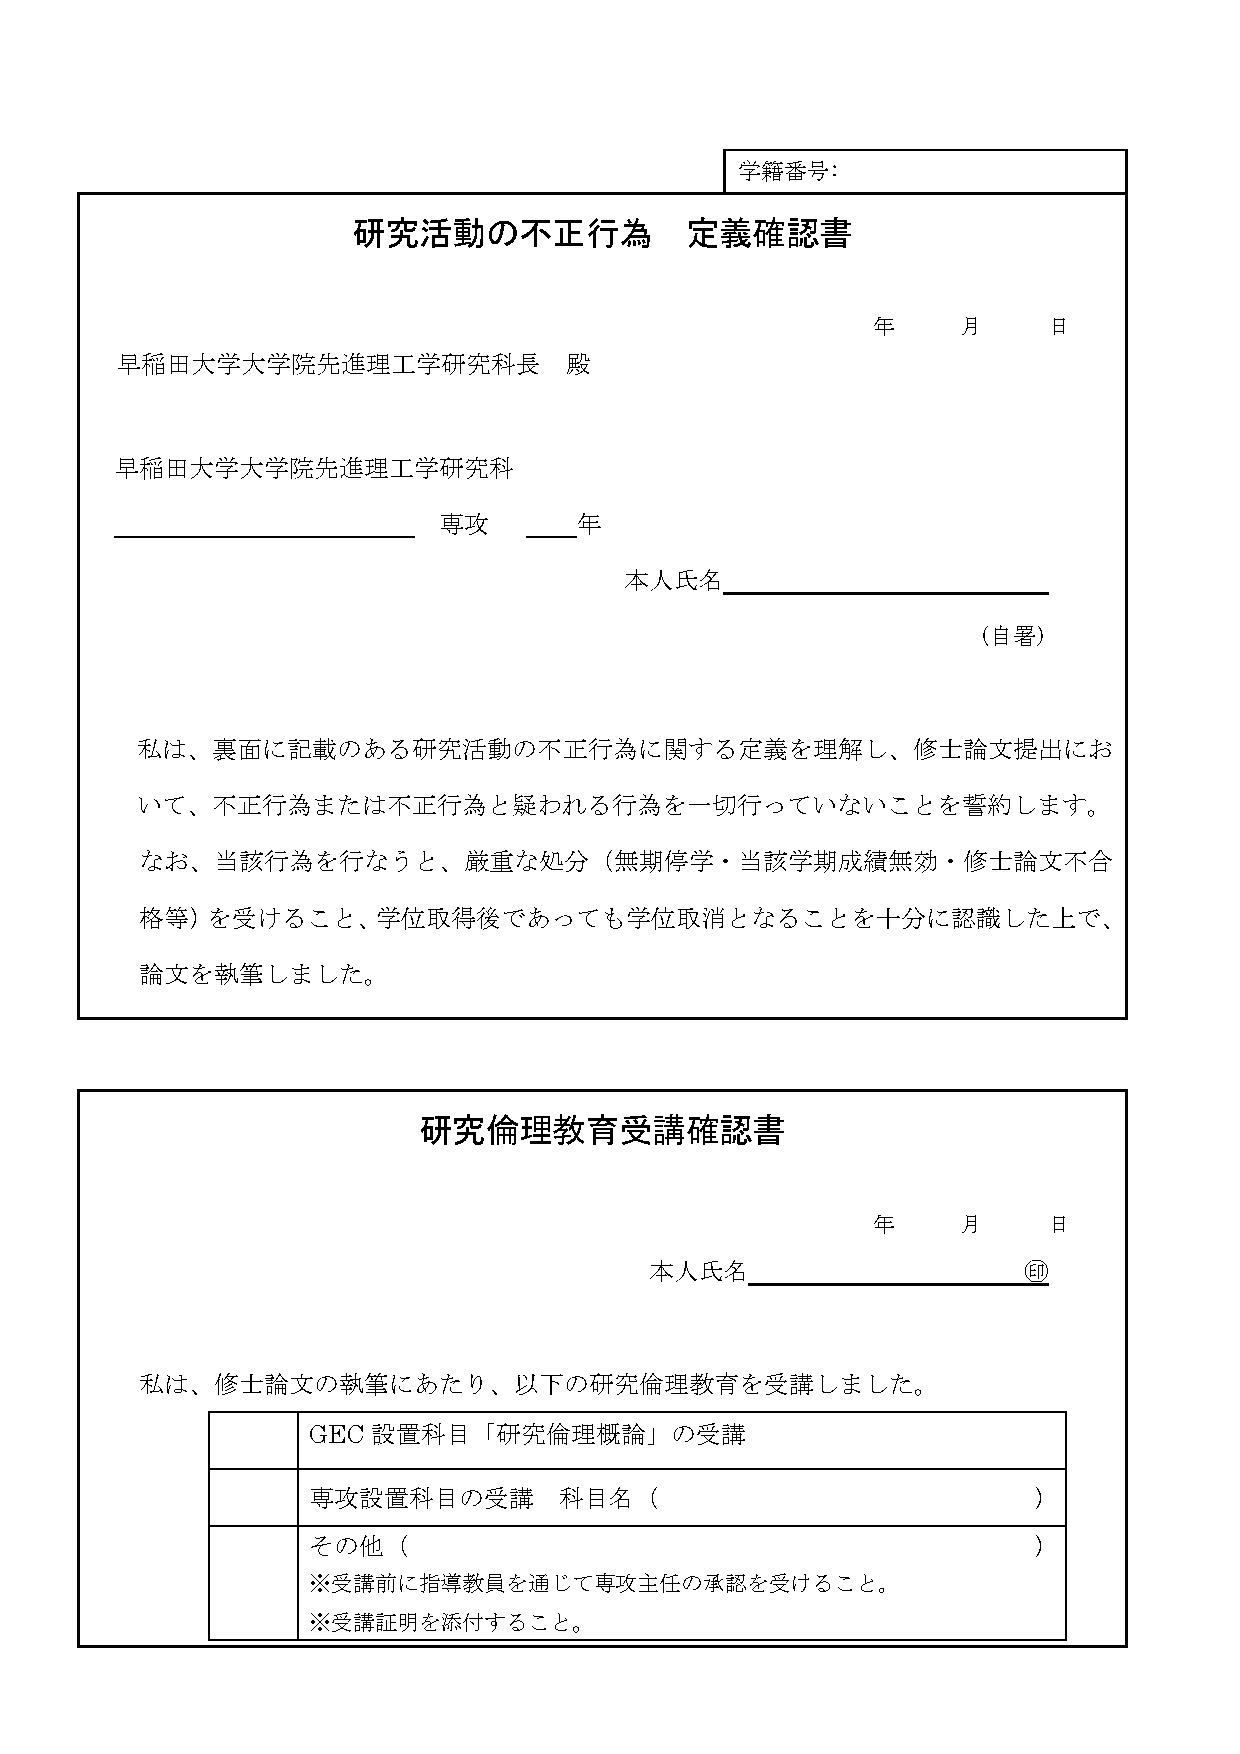
\includepdf[pages=-]{extra/seiyaku.pdf} % 誓約書

\end{document}
